\documentclass[conference]{IEEEtran}
\usepackage{cite,amsmath,graphicx,booktabs,url}
\pagestyle{plain}
\title{Operation-aware timing and size policies for DNP3\\Working Case 4 candidate}
\author{}
\begin{document}
\maketitle
\begin{abstract}
We develop a programmable-switch framework that uses operation knowledge to
schedule acknowledgments and responses and to change supported control-message
sizes. Case 4 combines response-ready scheduling with valid command-object
padding and response segmentation. Software endpoints accept the bounded padding
profile, and an isolated software switch executes the composition. The current
retained Tofino recovery snapshot compiles; revised source, transport translation
and the complete joint hardware implementation require fresh qualification.
This working draft
keeps those evidence levels separate from the frozen timing campaign.
\end{abstract}
% Paragraphs 1-3 are Dr. Lin's supplied text, installed VERBATIM on 2026-09-08. Only the
% bracketed reference numbers are mapped to bibliography keys; not one word is changed.
% Grammar, factual and citation concerns are recorded in
% pipeline/reports/POST_MEETING_REVIEW_HANDOFF.md, not corrected here.
% Paragraph 4 and the contributions are the framework/contribution continuation the meeting
% asked for; they are not protected text.
\section{Introduction}
\label{sec:intro}

Device fingerprinting has been an essential step in cyber reconnaissance, allowing adversaries
to reveal unique features of target networks and to design effective, stealthy attack
strategies. These techniques are becoming increasingly critical in industrial control systems
(ICSs) such as power grids, where adversaries often use IP-based control networks and computing
devices within as entry points to inflict physical damage. Consequently, fingerprinting shifts
the focus from visited websites and user biometric behavior to device models and types of
control operations that are critical to ICS attacks. In the 2015 attack that disrupted Ukrainian
power grids and the Stuxnet attack that disrupted Iranian nuclear power facilities, it is widely
believed that adversaries stayed in their systems for at least 6 months to perform cyber
reconnaissance~\cite{ukraine2015, stuxnet2011}.

To disrupt device fingerprinting, many studies have presented network traffic
obfuscation~\cite{wright2009, dyer2012}. Device
fingerprinting targeting general computing environments generally relies on network-level
features such as packet size and/or inter-packet latency observed from communication
patterns~\cite{sirinam2018}. Consequently, existing traffic
obfuscation often focuses on (i) padding and splitting network packets, which hide or change the
distribution of network packet sizes~\cite{wright2009, walkietalkie2017, panchenko2016}, and (ii)
delaying network packets and adding dummy ones, which disrupt the inter-packet timing
pattern~\cite{dyer2012, tamaraw2014, wang2008dlp, juarez2016}. Since manipulating
communication networks can introduce runtime overhead, recent works have begun to offload
traffic obfuscation onto programmable network switches, which change communication patterns at
much higher line rates than CPUs~\cite{ditto2022, minos2025, securitas2026}.

Unfortunately, these methods cannot be directly applied to ICS environments for two main
reasons. First, device fingerprinting methods on ICS devices rely on different features from the
ones in general computing environments. Instead of using network layer knowledge, they attempt
to use behavior on physical devices to reveal device model or types of operations. For example,
work in~\cite{formby2016, shen2018, ahmed2021, pospisil2023} uses the latency between the
TCP acknowledge packets and the actual response from the same device to estimate execution time
there. Since each
vendors may choose different materials or algorithms to implement the same control
functionality, this time can be accurate in fingerprinting those devices. Second, existing
traffic obfuscation is performed over encrypted channels, which are necessary to mix the
obfuscated and normal traffic. Unfortunately, ICS networks still rely on unencrypted traffic due
to a wide range of legacy devices, despite ICS network protocols may provide security features.
Directly padding or adding dummy packets can easily reveal obfuscated packets, exposing the the
underlying traffic pattern to adversaries.

In this paper, we develop an operation-aware framework for timing and size
policies on a programmable switch. The framework identifies protocol control
units and applies supported padding, splitting and scheduling policies while
retaining legitimate endpoint communication. Case 4 is the new implementation
target. Our current evidence establishes bounded software composition and a
compiled recovery component; the complete joint Tofino realization remains an
implementation gate. These claims require neither endpoint encryption nor
separate de-obfuscation hardware, and do not establish hidden device identity.

\section{Framework Design}
\textbf{Architecture.} The framework applies policies to the packets that carry
an operation. Ingress identifies the request, its TCP acknowledgment and its
application response. The traffic manager holds packets behind internal blocker
reservoirs. Returning packets pass through ingress again before they are released
or queued. Egress forwards a released packet or produces the supported response
segments. Blockers remain inside the switch; a cloned request triggers their
generation and is not itself a reservoir.

\begin{figure*}[t]
\centering
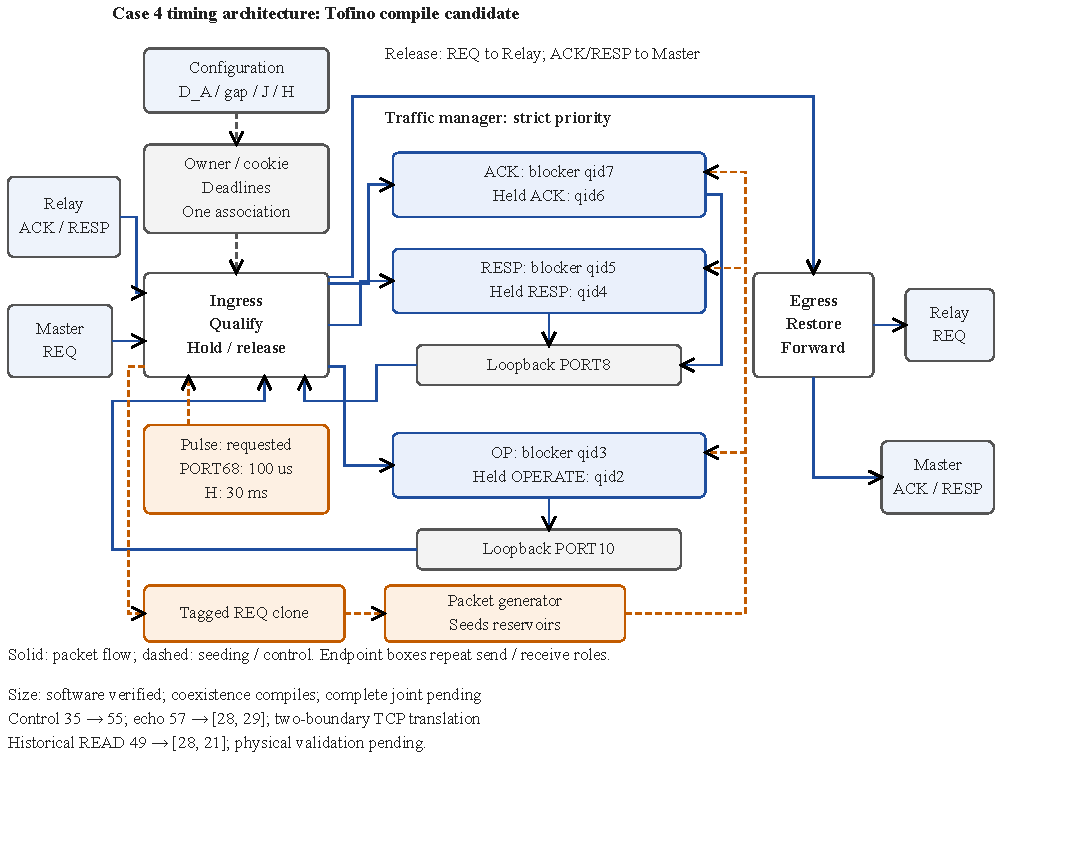
\includegraphics[width=\textwidth]{../figures/fig_framework_mechanism.pdf}
\caption{Working mechanism and separate size component. The read and control
scheduling domains return through ingress. The size branch is not evidence of a
complete joint Tofino implementation. Source, queue mapping and rendering
provenance accompany the editable figure.}
\label{fig:mechanism}
\end{figure*}

\textbf{Operation-related policies.} A response has a generic DNP3 RESPONSE
function, so the owner request determines its parent operation. READ, SELECT and
OPERATE remain separate populations. SELECT and OPERATE form two phases of
select-before-operate (SBO); a response segment inherits its parent's operation.
For an eligible control request, the size policy appends a configured inert
command object while retaining every real object and its fields. It repeats the
same transformation on the matching OPERATE. Response splitting changes TCP
segmentation, not the application message. The policy requires successful real
and decoy statuses and a verified inert-point configuration.

\textbf{Case 4 composition.} An early response waits until its acknowledgment
can leave. A late response becomes the readiness event for acknowledgment release.
After normal acknowledgment commitment, the response waits the full configured
gap. In an ideal schedule, with request arrival $t_0$, native acknowledgment
arrival $t_A$, complete associated response availability $t_R$, request-relative
acknowledgment deadline $D_A$, and physical departures $e_A,e_R$,
\begin{align}
e_A&=\max(t_0+D_A,t_A,t_R),\\
e_R&=e_A+\mathrm{configured\ CLRT}_{new}.
\end{align}
The acknowledgment hold is $e_A-t_A$, and the response hold is $e_R-t_R$.
Consequently, subtracting only the native acknowledgment-to-response interval
from $D_A$ omits the request-to-acknowledgment interval. The implementation starts
the response deadline at qualified loopback commitment, an internal reference
that remains distinct from measured physical departure.

\textbf{Finite recovery.} A 30 ms readiness expiry advances independently of
both reservoirs. If readiness fails, the switch releases held originals without
fabricating an acknowledgment or response. A normal ACK commitment invalidates
an in-flight readiness scan and preserves the future response deadline. Packet
ordering near expiry can still select explicit fallback before commitment.
Completion, stale-packet rejection and next-owner admission need separate checks;
an event-model timer does not establish physical queue drain.

\textbf{Parameter constraints.} Admission accounts for the complete feedback
interval each sender's timer spans, application and SBO deadlines, detection,
drain and release. TCP's retransmission timer is not remaining headroom at switch
arrival~\cite{case4_rfc6298}. Missing measurements keep admission provisional.
The policy study retains $D_A\in\{5,10,15,20\}$ ms and configured
$\mathrm{CLRT}_{new}=1$ ms, subject to a fixed 40 ms cap. The declared hardware
accuracy criteria are not software timing tolerances or achieved results.

\textbf{Other policy capabilities.} ACK-focused scheduling moves
request-to-ACK timing toward response readiness. Response-focused scheduling
holds only responses that arrive inside its window. A generated-ACK prototype
accepts responsibility for downstream loss and remains incomplete. These three
cases are explanation-only history in this assignment; Case 4 is the new target.

\section{Implementation}
The Tofino candidate extends the existing response-ready program. A single owner
stores TCP positions and the DNP3 application sequence. A separate periodic
internal pulse scans readiness and completion even if both blocker reservoirs
vanish. Held packets recheck eligibility; a second pass commits ACK-gap arming
or response retirement. A released-domain marker forwards OPERATE transport
repair after release, while the configured-session predicate isolates control
state. The current build identity and resource reports are recorded in the
canonical capability matrix. Compilation does not establish packet-generator
service, wire departure, queue drain or live restoration.

The software size oracle validates complete DNP3 frames and regenerates their
link CRCs. One native control command has a 35-byte TCP payload; appending a
separate Group 12 Variation 1 header and one object produces 55 bytes. Its native
response is 37 bytes, while the accepted padded response is 57 bytes. The added
application bytes cross a CRC-block boundary, making the request-stream delta
20 bytes. The response policy splits that exact 57-byte profile into 28 and
29 bytes. The historical 49-byte profile remains a separate 28/21 carve.

Insertion changes the TCP byte space. The software ledger retains two original
and rewritten request images for one SELECT/OPERATE pair. It replays rewritten
bytes on whole, partial and overlapping retransmissions and inverts cumulative
or partial acknowledgment positions. An acknowledgment inside an inserted tail
keeps the last native byte outstanding until the complete wire image is
acknowledged; replay of that byte supplies the cached missing suffix. It maps
the unscaled receive-window right
edge through the same transformation~\cite{case4_rfc9293}. It continues existing
translation after insertion capacity is reached. Unsupported negotiated
features must exclude insertion before bytes change; a feature refusal after
insertion cannot erase the ledger.

The BMv2 artifact uses private namespaces and Python codec endpoints. Its token
count gates and recirculating real held packets emulate the blocker principle;
they do not reproduce Tofino's queue server. The software heartbeat is 1 ms,
separate from the proposed 100 microsecond hardware pulse. We use the BMv2
architecture documentation to identify those interfaces~\cite{case4_bmv2}.
An independent pinned OpenDNP3 master/outstation gate tests production command
serialization, SBO state and statuses~\cite{case4_opendnp3}. These endpoint
contexts are not the Python endpoints of the namespace experiment.

\section{Evaluation}
\textbf{Measurement boundary.} We distinguish the frozen physical timing
campaign, the historical Timing OFF smoke, the production-stack semantic gate,
packet simulations and the current namespace switch. The frozen campaign has
63,360 exchanges in 22 grouped runs and uses request-anchored 20/8 ms timing with
size processing off. It is not a measurement of Case 4 padding or current
response-ready recovery. The OFF smoke contains 30 main 49-byte READ responses
and one separate 58-byte precheck. The main cohort's master-facing median CLRT
is 2.232 ms, with a range from 1.104 to 22.387 ms. A master-facing capture does
not identify the outstation's transmission endpoint or full response latency
$D_R$.

\textbf{Endpoint acceptance.} The isolated production-stack gate accepts the
trailing-header command profile and returns SUCCESS for the real and decoy
objects in both phases. It also exposes a failure that a parser-only test misses:
the unmodified master ignores a failed trailing decoy SELECT and still emits
OPERATE. The outstation then returns NO\_SELECT and performs no command callback.
Thus receipt of a matching OPERATE response cannot replace per-object status
checks. These callbacks are software events, not evidence of physical inertness.

\textbf{Timing and stream behavior.} Source-driven packet tests compare actual
association inputs, owner actions and constant tables with the event model.
Namespace tests verify insertion, translation, CRCs, reassembly and application
outcomes on captured packets. Exact test counts, failures and skips belong to the
retained verification record. Software timing has scheduling excursions and is
not compared with the hardware microsecond acceptance criteria. Historical
120-READ populations keep all seven below-target observations; focused and
full-range histograms retain the complete attempted denominators.

\textbf{Cost and resource boundary.} Recovery has a source-bound local Tofino
compile. Fixed size processing has a component compile, while the complete
two-boundary transport implementation encounters target PHV/action limits.
Component coexistence is not a complete joint fit. The controller refuses
activation when joint schema, byte translation, applicable timers or measured
release costs are missing. The proposed run list has 16,168 attempts, including
warmups and state checks, under the 18,360-attempt ceiling. No new hardware
campaign has been collected for this candidate.

\subsection{Limitations}
Full-frame CRC admission, connection-epoch quarantine, immediate matching
FIN/RST flush and drain before owner reuse remain incomplete in the Tofino
recovery component. Control command hold needs source-current packet and
hardware coverage. Normal commitment near readiness expiry can lose to explicit
fallback, even if the ideal model sees a response just before expiry. Current
hardware timing inputs remain unavailable. The software ledger and namespace
tests do not close the target translation fit. Plaintext function codes and
object identities remain visible; matching sizes and compressed CLRT do not
establish hidden device identity or reconnaissance prevention.

Formby et al. form device signatures from CLRT histogram counts with a heuristic
overflow threshold~\cite{formby2016}. Our existing software populations have no
device labels. We therefore export features with negative, exact-threshold and
overflow accounting without reporting device classification accuracy or a
uniform chance baseline. No classifier result is inferred from reduced variance.

\bibliographystyle{IEEEtran}
\bibliography{References,case4_refs}
\end{document}
